\textbf{Agenda}

Pada Bab ini kita akan mempelajari tentang module bawaan Qt Creator yaitu
Qt Webkit seperti berikut ini

\minitoc

\section{Qt Webkit}\label{qt-webkit}

Pada contoh ini kita akan membuat sebuah browser dengan menggunakan 
Qt Webkit 

pertama,kita akan mencoba memuat sebuah url untuk menampilkan halaman
kemudian 
First, we'll just try to load a url to display a web page, then start to
build the more refined browser.

In my opinion, one of the most important pieces of Qt Webkit is
QWebView. The Qt document also says:

\begin{quote}
Qwebview merupakan komponen widget utama dari module web browser Qtwebkit
yang dapat digunakan dalam beberapa aplikasi untuk menampilkan konten
pada internet 
\end{quote}

\subsubsection*{Contoh membuat browser dengan Qt Webkit dengan meload url}\label{my-web-browser-version-1}

Sebuah website dapat di muat kedalam sebuah browser dengan menggunakan Qwebview 
dengan fungsi load() fungsi ini merupakan bagian core dari peting untuk menampilkan 
konten statis pada browser

\begin{lstlisting}[language=c++, numbers=none]
QWebView *view = new QWebView(parent);
view->load(QUrl("http://google.com/"));
view->show();
\end{lstlisting}

We make a QWebView object, and load a page using load(). Like all Qt
widgets, to display QWebView, the show() function must be invoked.

To make it work, we need a module from webkit (actually, webkitwidgets),
and we will set it in .pro file.

Though it's not necessary for this simple project, we'll use Creator.

File-\textgreater{}New File or Project\ldots{}-\textgreater{}Other
Project-\textgreater{}Empty Qt Project-\textgreater{}Choose\ldots{}

\begin{figure}[htbp]
\centering
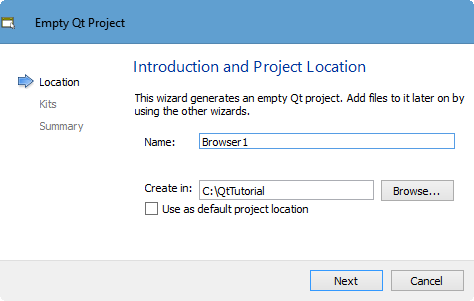
\includegraphics[width=0.8\textwidth]{../manuscript/images/Browser1_Empty_Project}
\caption{}
\end{figure}

Paste the following lines to the Browser1.pro:

\begin{lstlisting}[language=c++, numbers=none]
QT       += core gui
QT       += webkitwidgets

greaterThan(QT_MAJOR_VERSION, 4): QT += widgets

TARGET = Browser1
TEMPLATE = app

SOURCES += main.cpp
Then we need a main().
\end{lstlisting}

Right click on the Project name and select Add
new\ldots{}-\textgreater{}C++-\textgreater{}C++ Source
File-\textgreater{}Choose\ldots{}


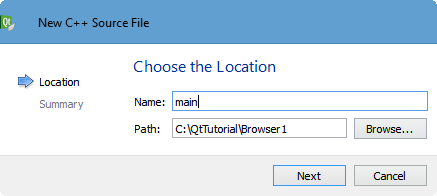
\includegraphics[width=0.8\textwidth]{../manuscript/images/main_cpp}

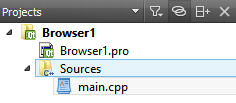
\includegraphics[width=0.8\textwidth]{../manuscript/images/Browser1_files}


Copy the following code for the main.cpp:

\begin{lstlisting}[language=c++, numbers=none]
#include <QApplication>
#include <QWebView>

int main(int argc, char *argv[])
{
    QApplication a(argc, argv);
    QWebView view;
    view.show();
    view.load(QUrl("http://google.com"));

    return a.exec();
}
\end{lstlisting}

Run qmake-\textgreater{}Run, then we'll get our browser with the page
loaded:

\begin{figure}[htbp]
\centering
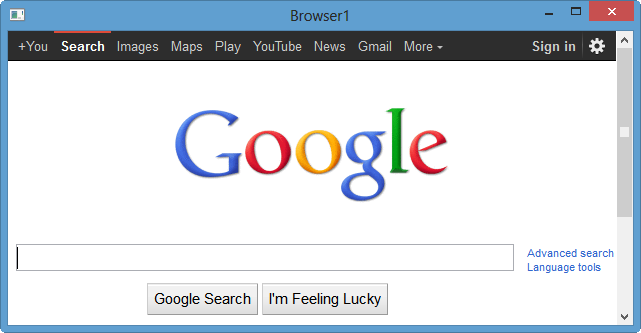
\includegraphics[width=0.8\textwidth]{../manuscript/images/Browser1_Run}
\caption{}
\end{figure}

NOTE: The linking against the Webkit does not seem to be needed. So, I
dropped the following line from the Browser1.pro file.

\begin{lstlisting}[language=c++, numbers=none]
QT       += webkit
\end{lstlisting}

\section{My Web Browser version 2}\label{my-web-browser-version-2}

Though our browser version 1 is able to display a page, it does not have
controls such as backward, forward, or refresh etc.

So, in the next tutorial, we'll put some UI elements so that our browser
become more closer to the real one.

\subsection{Starting the Project}\label{starting-the-project}

Right click on the Project name and select Add
new\ldots{}-\textgreater{}Applications-\textgreater{}Qt Gui
Application-\textgreater{}Choose\ldots{}

(Note) Depending on the version, we may want to select Add
new\ldots{}-\textgreater{}Qt-\textgreater{}Qt Designer Form
Class-\textgreater{}Dialog without Buttons

\begin{figure}[htbp]
\centering
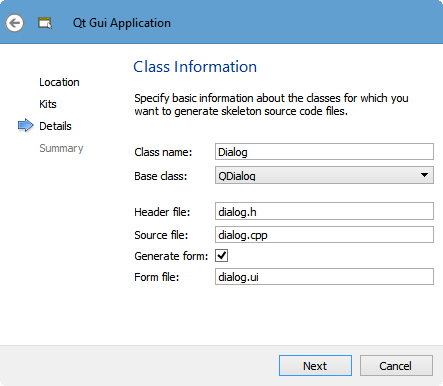
\includegraphics[width=0.8\textwidth]{../manuscript/images/QDialog}
\caption{}
\end{figure}

\begin{figure}[htbp]
\centering
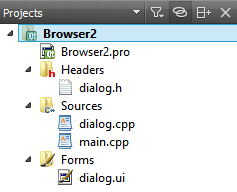
\includegraphics[width=0.8\textwidth]{../manuscript/images/Browser2_Files}
\caption{}
\end{figure}

.pro File To link against Webkit, we need to add one line to the .pro
file (with Qt5.3, the line will be added automatically):

\begin{lstlisting}[language=c++, numbers=none]
QT       += core gui
QT       += webkitwidgets

greaterThan(QT_MAJOR_VERSION, 4): QT += widgets

TARGET = Browser2
TEMPLATE = app


SOURCES += main.cpp\
        dialog.cpp

HEADERS  += dialog.h

FORMS    += dialog.ui
\end{lstlisting}

\subsection{Working on UI}\label{working-on-ui}

Let's add ``urlEdit,''backButton``,''forwardButton``,''refreshButton,
and ``goButton''. Also the key widget which is ``webView'' for QWebView:

\begin{figure}[htbp]
\centering
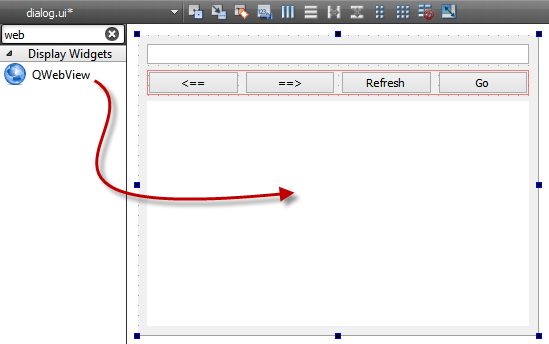
\includegraphics[width=0.8\textwidth]{../manuscript/images/AddingWebView}
\caption{}
\end{figure}

Slots for the buttons and urlEdit To make the Creator to write a code
for us, right click on the ``backButton''-\textgreater{}GO to
slot\ldots{}-\textgreater{}clicked()

\begin{figure}[htbp]
\centering
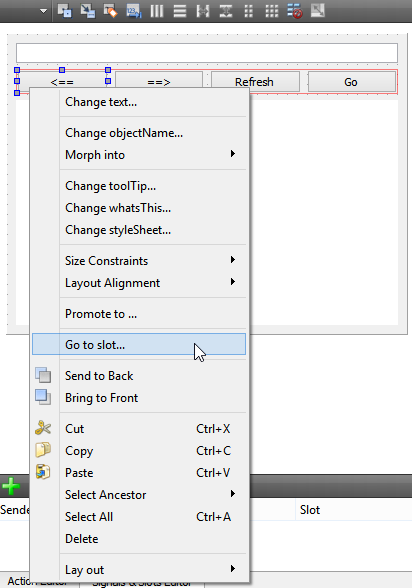
\includegraphics[width=0.8\textwidth]{../manuscript/images/GoToSlotBrowser}
\caption{}
\end{figure}

Then, in the dialog.cpp, it will write a slot function for us for the
``backButton'' click:

void Dialog::on\_backButton\_clicked() \{

\} Also, the Creator will write the prototype declaration into the
dialog.h as well.

We need to do the same for the other three buttons.

For the ``urlEdit'' button, we may want to select returnPressed(),
instead.

\section{Writing Code for the
Slots}\label{writing-code-for-the-slots}

We need to tell our Browser what to do when those buttons are clicked or
return key is pressed on the urlEdit.

First we need to include QWebView into the dialog.h.

Then, let's start coding for the to-do list.

Fortunately, the Creator intelligence gives us some hints on what to do:

\begin{figure}[htbp]
\centering
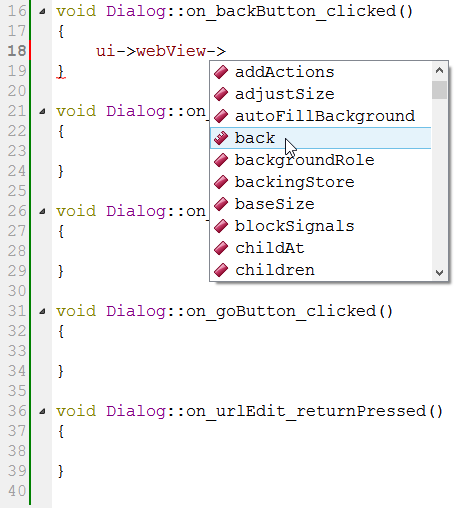
\includegraphics[width=0.8\textwidth]{../manuscript/images/BackButtonCoding}
\caption{}
\end{figure}

So, the finished coding, our slots in dialog.cpp look like this:

\begin{lstlisting}[language=c++, numbers=none]
void Dialog::on_backButton_clicked()
{
    ui->webView->back();
}

void Dialog::on_forwardButton_clicked()
{
    ui->webView->forward();
}

void Dialog::on_refreshButton_clicked()
{
    ui->webView->reload();
}

void Dialog::on_goButton_clicked()
{
    // We just type the domain without "http://"
    ui->webView->load(("http://"+ui->urlEdit->text()));
}

void Dialog::on_urlEdit_returnPressed()
{
    // Same as goButton click
    on_goButton_clicked();
}
\end{lstlisting}

\subsection{Running the Code}\label{running-the-code}

Let's run our code.

\begin{figure}[htbp]
\centering
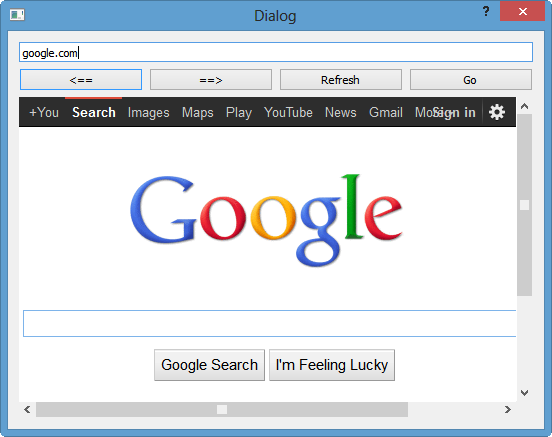
\includegraphics[width=0.8\textwidth]{../manuscript/images/Browser2RunA}
\caption{}
\end{figure}

If we type in another site:

\begin{figure}[htbp]
\centering
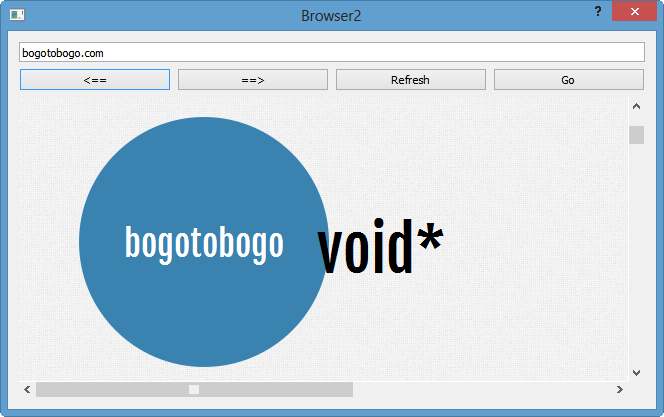
\includegraphics[width=0.8\textwidth]{../manuscript/images/Browser2RunB}
\caption{}
\end{figure}

\subsection{Source Code}\label{source-code}

Here is the source code: Browser2.zip.

\begin{lstlisting}[language=c++, numbers=none]
main.cpp.

#include "dialog.h"
#include <QApplication>

int main(int argc, char *argv[])
{
    QApplication a(argc, argv);
    Dialog w;
    w.setWindowTitle("Browser2");
    w.show();

    return a.exec();
}
\end{lstlisting}

dialog.h.

\begin{lstlisting}[language=c++, numbers=none]
#ifndef DIALOG_H
#define DIALOG_H

#include <QDialog>
#include <QWebView>

namespace Ui {
class Dialog;
}

class Dialog : public QDialog
{
    Q_OBJECT

public:
    explicit Dialog(QWidget *parent = 0);
    ~Dialog();

private slots:
    void on_backButton_clicked();

    void on_forwardButton_clicked();

    void on_refreshButton_clicked();

    void on_goButton_clicked();

    void on_urlEdit_returnPressed();

private:
    Ui::Dialog *ui;
};

#endif // DIALOG_H
\end{lstlisting}

dialog.cpp.

\begin{lstlisting}[language=c++, numbers=none]
#include "dialog.h"
#include "ui_dialog.h"

Dialog::Dialog(QWidget *parent) :
    QDialog(parent),
    ui(new Ui::Dialog)
{
    ui->setupUi(this);
}

Dialog::~Dialog()
{
    delete ui;
}

void Dialog::on_backButton_clicked()
{
    ui->webView->back();
}

void Dialog::on_forwardButton_clicked()
{
    ui->webView->forward();
}

void Dialog::on_refreshButton_clicked()
{
    ui->webView->reload();
}

void Dialog::on_goButton_clicked()
{
    // We just type the domain without "http://"
    ui->webView->load(("http://"+ui->urlEdit->text()));
}

void Dialog::on_urlEdit_returnPressed()
{
    // Same as goButton click
    on_goButton_clicked();
}
\end{lstlisting}

There are lots of things to be done to make our browser better.
